\documentclass[11pt]{article}

\usepackage[T1]{fontenc}
\usepackage[utf8]{inputenc}
\usepackage{lmodern}
\usepackage{microtype}
\usepackage[margin=1in]{geometry}
\usepackage{amsmath,amssymb,amsthm,mathtools}
\usepackage{booktabs}
\usepackage{tabularx}
\usepackage{longtable}
\usepackage{array}
\usepackage{enumitem}
\usepackage{xcolor}
\usepackage{tcolorbox}
\usepackage{tikz}
\usepackage{pgfplots}
\usepackage{fancyhdr}
\usepackage{hyperref}
\usepackage[nameinlink,noabbrev]{cleveref}

\pgfplotsset{compat=1.18}
\usetikzlibrary{arrows.meta,positioning}

\definecolor{navy}{HTML}{17365D}
\definecolor{blue}{HTML}{2E75B6}
\definecolor{lightblue}{HTML}{EAF3F8}
\definecolor{orange}{HTML}{C55A11}
\definecolor{lightorange}{HTML}{FCEDE3}
\definecolor{green}{HTML}{548235}
\definecolor{lightgreen}{HTML}{EEF5E9}
\definecolor{graytext}{HTML}{4A4A4A}
\definecolor{lightgray}{HTML}{F4F5F7}

\hypersetup{
  colorlinks=true,
  linkcolor=navy,
  citecolor=green,
  urlcolor=blue,
  pdftitle={From Bernoulli Outcomes to Binary Cross-Entropy},
  pdfsubject={Lecture notes on logistic regression and cross-entropy},
  pdfauthor={Paul Agraon}
}

\pagestyle{fancy}
\fancyhf{}
\lhead{Binary Cross-Entropy and Logistic Regression}
\rhead{Lecture Notes}
\cfoot{\thepage}
\setlength{\headheight}{14pt}

\setcounter{secnumdepth}{3}
\setcounter{tocdepth}{2}
\setlist[itemize]{topsep=4pt,itemsep=2pt}
\setlist[enumerate]{topsep=4pt,itemsep=3pt}
\renewcommand{\arraystretch}{1.18}
\newcommand{\rowrule}{\specialrule{0.20pt}{1.25pt}{1.25pt}}

\newcommand{\R}{\mathbb{R}}
\newcommand{\E}{\mathbb{E}}
\newcommand{\Prob}{\mathbb{P}}
\newcommand{\sigmoid}{\sigma}
\newcommand{\given}{\,\middle|\,}
\newcommand{\BCE}{\operatorname{BCE}}
\newcommand{\KL}{D_{\mathrm{KL}}}
\newcommand{\softplus}{\operatorname{softplus}}

\newtcolorbox{keyidea}[1][]{
  colback=lightblue,
  colframe=blue,
  boxrule=0.7pt,
  arc=2pt,
  left=7pt,right=7pt,top=6pt,bottom=6pt,
  title={#1},
  fonttitle=\bfseries
}

\newtcolorbox{warningbox}[1][]{
  colback=lightorange,
  colframe=orange,
  boxrule=0.7pt,
  arc=2pt,
  left=7pt,right=7pt,top=6pt,bottom=6pt,
  title={#1},
  fonttitle=\bfseries
}

\newtcolorbox{examplebox}[1][]{
  colback=lightgreen,
  colframe=green,
  boxrule=0.7pt,
  arc=2pt,
  left=7pt,right=7pt,top=6pt,bottom=6pt,
  title={#1},
  fonttitle=\bfseries
}

\theoremstyle{definition}
\newtheorem{definition}{Definition}[section]
\newtheorem{proposition}{Proposition}[section]

\title{\vspace{-1.5cm}\textbf{From Bernoulli Outcomes to Binary Cross-Entropy}\\[4pt]
\large Why Logistic Regression Uses Log Loss}
\author{Paul Agraon\\[3pt]\normalsize Lecture Notes in Machine Learning and Statistics}
\date{}

\begin{document}

\maketitle

\begin{abstract}
Binary cross-entropy is often presented as a formula to memorize. This article instead derives it from a sequence of modeling decisions: binary outcomes are described by a Bernoulli distribution; logistic regression assigns a conditional Bernoulli probability to each label; maximum likelihood selects parameters that make the observed labels probable; and logarithms convert independent probability products into additive evidence. We then connect the resulting negative log-likelihood to cross-entropy, entropy, Kullback--Leibler divergence, gradients, convex optimization, and numerically stable computation. Along the way, we distinguish probability from likelihood, a realized log loss from an expected cross-entropy, and the conceptual reason for logarithms from their computational advantages.
\end{abstract}

\vspace{0.75em}

\begin{keyidea}[The central statement]
For Bernoulli logistic regression,
\[
\boxed{\text{binary cross-entropy}
=\text{negative Bernoulli log-likelihood}}
\]
The Bernoulli model does \emph{not} itself contain a logarithm. The logarithm enters when we score or optimize the likelihood. It is the natural functional form when independent probabilities multiply but their information, evidence, or loss should add.
\end{keyidea}

\paragraph{Learning objectives.}
After reading these notes, a student should be able to:
\begin{itemize}
  \item define the Bernoulli model, logit, sigmoid, likelihood, log-likelihood, entropy, cross-entropy, and KL divergence;
  \item derive binary cross-entropy from maximum likelihood;
  \item explain why a logarithm is conceptually natural, not merely numerically convenient;
  \item interpret one-observation log loss and dataset-average cross-entropy;
  \item derive the gradient $p-y$ and explain its optimization behavior; and
  \item implement the loss stably from logits without evaluating $\log(0)$.
\end{itemize}

\begingroup
\small
\tableofcontents
\endgroup
\newpage

\section{The modeling problem}

We observe a dataset
\[
\mathcal{D}=\{(x_i,y_i)\}_{i=1}^{n},
\]
where $x_i\in\R^d$ is a vector of predictors and $y_i\in\{0,1\}$ is a binary label. Examples include whether a patient has a disease, whether a customer defaults, or whether an email is spam.

Logistic regression does not directly predict the class label. It first produces a real-valued \emph{linear score}
\begin{equation}
z_i=w^\top x_i+b,
\label{eq:linear-score}
\end{equation}
and converts it into a probability with the sigmoid function:
\begin{equation}
p_i=\sigmoid(z_i)=\frac{1}{1+e^{-z_i}}.
\label{eq:sigmoid}
\end{equation}
The model interprets this number as
\[
p_i=\Prob(Y_i=1\mid x_i;w,b),
\qquad
1-p_i=\Prob(Y_i=0\mid x_i;w,b).
\]

The score $z_i$ is also called the \emph{logit}. Indeed,
\begin{equation}
\log\frac{p_i}{1-p_i}=z_i=w^\top x_i+b.
\label{eq:logodds}
\end{equation}
Thus logistic regression assumes that the \emph{log-odds} of class 1 are linear in the predictors. The odds are $p/(1-p)$; the logit is the natural logarithm of those odds.

\begin{center}
\begin{tabularx}{0.94\textwidth}{>{\raggedright\arraybackslash}p{0.18\textwidth} X}
\toprule
\textbf{Term} & \textbf{Meaning in this article} \\
\midrule
Score / logit $z$ & Unbounded raw output $w^\top x+b$ before the sigmoid. \\
\rowrule
Probability $p$ & Model prediction $\Prob(Y=1\mid x;w,b)=\sigmoid(z)$. \\
\rowrule
Odds & Ratio $p/(1-p)$ of class-1 probability to class-0 probability. \\
\rowrule
Label $y$ & Observed outcome, equal to either 0 or 1. \\
\rowrule
Parameters $\theta$ & Model quantities being fitted; here $\theta=(w,b)$. \\
\bottomrule
\end{tabularx}
\end{center}

\section{The Bernoulli model}

\subsection{One binary observation}

A Bernoulli random variable has two possible outcomes. If
\[
Y\sim\operatorname{Bernoulli}(p),
\]
then
\[
\Prob(Y=1)=p,
\qquad
\Prob(Y=0)=1-p.
\]
Both cases can be written in one probability mass function:
\begin{equation}
\boxed{\Prob(Y=y\mid p)=p^y(1-p)^{1-y}},
\qquad y\in\{0,1\}.
\label{eq:bernoulli-pmf}
\end{equation}
The exponents are switches. If $y=1$, then
\[
p^1(1-p)^0=p;
\]
if $y=0$, then
\[
p^0(1-p)^1=1-p.
\]

In logistic regression, $p$ is not one constant shared by every observation. It depends on the predictors:
\[
Y_i\mid x_i\sim\operatorname{Bernoulli}(p_i),
\qquad p_i=\sigmoid(w^\top x_i+b).
\]
This is a \emph{conditional Bernoulli model}.

\subsection{Probability versus likelihood}

The same mathematical expression can be viewed in two different ways:
\begin{align*}
\Prob(Y=y\mid p)& &&\text{varies the possible data $y$ while $p$ is fixed},\\
L(p;y)&=p^y(1-p)^{1-y} &&\text{varies the parameter $p$ while observed $y$ is fixed}.
\end{align*}
The first is a probability mass function. The second is a \emph{likelihood function}. A likelihood is not a probability distribution over the parameter unless additional Bayesian machinery supplies a prior and normalization.

\begin{warningbox}[A crucial distinction]
Maximum likelihood does not ask, ``What is the probability that these parameters are correct?'' It asks, ``If these parameters were used by the data-generating model, how much probability would that model assign to the data we observed?''
\end{warningbox}

\section{One observation: log loss and cross-entropy}

Suppose the model predicts $p=\Prob(Y=1\mid x)$ and the observed label is $y$. The probability assigned to the outcome that actually occurred is
\begin{equation}
r=p^y(1-p)^{1-y}
=
\begin{cases}
p,&y=1,\\
1-p,&y=0.
\end{cases}
\label{eq:correct-prob}
\end{equation}
The one-observation \emph{log loss} is
\begin{equation}
\ell(y,p)=-\log r
=-\left[y\log p+(1-y)\log(1-p)\right].
\label{eq:bce-one}
\end{equation}
This is the familiar binary cross-entropy formula.

\subsection{What does this number measure?}

The quantity $-\log r$ is called the \emph{surprisal} or \emph{self-information} of an event to which the model assigned probability $r$. A likely event carries little surprise; an event the model considered nearly impossible carries a great deal.

\begin{center}
\begin{tabular}{rrl}
\toprule
$r$: probability assigned to what occurred & $-\ln r$ & Interpretation \\
\midrule
$0.99$  & $0.010$ & almost unsurprising \\
\rowrule
$0.90$  & $0.105$ & small loss \\
\rowrule
$0.50$  & $0.693$ & complete binary uncertainty \\
\rowrule
$0.10$  & $2.303$ & large loss \\
\rowrule
$0.01$  & $4.605$ & very large loss \\
\rowrule
$0.001$ & $6.908$ & extreme surprise \\
\bottomrule
\end{tabular}
\end{center}

The loss does \emph{not} measure ordinary geometric distance such as $|y-p|$. It evaluates the quality of a probabilistic forecast by asking how much probability the forecast assigned to the outcome that occurred.

\subsection{Why the term cross-entropy?}

Represent the observed label as a point-mass distribution over classes 0 and 1:
\[
Q_y=(1-y,y),
\]
and represent the model prediction as
\[
P_p=(1-p,p).
\]
For two discrete distributions $Q$ and $P$, their cross-entropy is
\begin{equation}
H(Q,P)=-\sum_c Q(c)\log P(c).
\label{eq:cross-entropy-general}
\end{equation}
Substitution gives
\[
H(Q_y,P_p)
=-\left[(1-y)\log(1-p)+y\log p\right],
\]
which is exactly \cref{eq:bce-one}.

\begin{keyidea}[Precise terminology]
For one realized label, $-\log P_p(y)$ is most precisely called the \emph{realized logarithmic score} or \emph{one-observation log loss}. It is also the cross-entropy between the model distribution and the empirical point mass placed on that observed label. Cross-entropy in the population sense is an \emph{expectation} over possible outcomes; we develop that distinction in \cref{sec:information-theory}.
\end{keyidea}

\section{Why logarithms are the natural choice}
\label{sec:why-log}

There are three related answers. Numerical convenience is only the third.

\subsection{Independent probabilities multiply}

Suppose two events $A$ and $B$ are independent and the model assigns them probabilities $p$ and $q$. Then
\[
\Prob(A\cap B)=pq.
\]
If a numerical measure $I(p)$ is to represent the information or surprise of observing an event of probability $p$, a natural consistency requirement is
\begin{equation}
I(pq)=I(p)+I(q).
\label{eq:additivity}
\end{equation}
In words: independent evidence should add even though independent probabilities multiply.

The logarithm has exactly this property:
\[
\log(pq)=\log p+\log q.
\]
Because smaller probabilities should produce larger positive surprise, the sign is reversed:
\begin{equation}
\boxed{I(p)=-k\log p},\qquad k>0.
\label{eq:self-information}
\end{equation}

\begin{proposition}[Uniqueness of logarithmic surprise]
Suppose $I:(0,1]\to\R$ is continuous, $I(1)=0$, less probable events have no less surprise, and independent surprises add as in \cref{eq:additivity}. Then $I(p)=-k\ln p$ for some $k>0$.
\end{proposition}

\paragraph{Proof sketch.}
Write $p=e^{-t}$ for $t\ge 0$ and define $g(t)=I(e^{-t})$. Then
\[
g(s+t)=I(e^{-s}e^{-t})=g(s)+g(t).
\]
The continuous solutions to this additive functional equation are $g(t)=kt$. Consequently,
\[
I(p)=g(-\ln p)=-k\ln p.
\]
Monotonicity requires $k>0$. \hfill$\square$

Thus the logarithm is not merely a convenient curve chosen to punish mistakes. Under these ordinary requirements, its functional form is essentially forced. This is the foundation of Shannon information theory \cite{shannon1948}.

\subsection{The base of the logarithm}

The logarithmic \emph{form} is fundamental; the base is a choice of units:
\begin{itemize}
  \item $\log_2$ measures information in \emph{bits};
  \item $\ln$ measures information in \emph{nats};
  \item any other base differs only by a positive constant factor.
\end{itemize}
Since
\[
\log_b p=\frac{\ln p}{\ln b},
\]
changing the base rescales every loss by the same positive constant and does not change the minimizing parameters. The natural logarithm is standard in statistics and optimization because its derivatives are simplest. Therefore, ``the logarithm is natural'' and ``the natural logarithm is mandatory'' are different claims: the first is conceptually justified; the second is false.

\subsection{Logarithms preserve the optimum and improve computation}

The logarithm is strictly increasing, so
\[
a>b\quad\Longleftrightarrow\quad \log a>\log b.
\]
Maximizing a positive likelihood and maximizing its logarithm therefore give exactly the same optimizer. The logarithm also turns products into sums, simplifies derivatives, and prevents products of many small probabilities from numerically underflowing to zero.

\section{Maximum likelihood}

\begin{definition}[Maximum likelihood principle]
Choose the parameter value that makes the observed data have the greatest probability under the assumed model:
\[
\widehat\theta_{\mathrm{MLE}}
=\arg\max_\theta L(\theta;\mathcal D)
=\arg\max_\theta \Prob(\mathcal D\mid\theta).
\]
\end{definition}

\subsection{Coin-flip example}

Suppose a coin is flipped $n=10$ times and the observed sequence contains $k=8$ heads and $2$ tails. If flips are independent with head probability $p$, the likelihood of the particular observed sequence is
\[
L(p)=p^8(1-p)^2.
\]
If we record only the count rather than the sequence, the binomial probability includes $\binom{10}{8}$, but that factor does not depend on $p$ and therefore does not change the maximum-likelihood estimate.

The log-likelihood is
\[
\ell(p)=8\log p+2\log(1-p).
\]
Differentiating and setting the result to zero,
\[
\ell'(p)=\frac{8}{p}-\frac{2}{1-p}=0
\quad\Longrightarrow\quad
8(1-p)=2p
\quad\Longrightarrow\quad
\widehat p=0.8.
\]
More generally, the Bernoulli MLE is the observed fraction of ones, $\widehat p=k/n$.

\subsection{Likelihood for a logistic-regression dataset}

Logistic regression normally assumes that labels are \emph{conditionally independent given their predictors and the parameters}. Therefore,
\begin{equation}
L(w,b)
=\prod_{i=1}^{n}\Prob(Y_i=y_i\mid x_i;w,b)
=\prod_{i=1}^{n}p_i^{y_i}(1-p_i)^{1-y_i}.
\label{eq:dataset-likelihood}
\end{equation}
Taking logarithms yields
\begin{equation}
\log L(w,b)
=\sum_{i=1}^{n}\left[y_i\log p_i+(1-y_i)\log(1-p_i)\right].
\label{eq:log-likelihood}
\end{equation}
Machine learning usually expresses fitting as loss minimization rather than likelihood maximization. Negating \cref{eq:log-likelihood} gives the negative log-likelihood (NLL):
\begin{equation}
\operatorname{NLL}(w,b)
=-\sum_{i=1}^{n}\left[y_i\log p_i+(1-y_i)\log(1-p_i)\right].
\label{eq:nll}
\end{equation}
Dividing by $n$ gives the mean binary cross-entropy:
\begin{equation}
\boxed{
\BCE(w,b)
=-\frac{1}{n}\sum_{i=1}^{n}
\left[y_i\log p_i+(1-y_i)\log(1-p_i)\right].}
\label{eq:bce-dataset}
\end{equation}
For a fixed dataset and no additional penalty, the sum and mean have the same minimizer. They differ only by a factor of $n$. If a regularization term is added, however, the convention matters because it changes the relative scale of the data loss and penalty.

\begin{keyidea}[The complete logical chain]
\centering
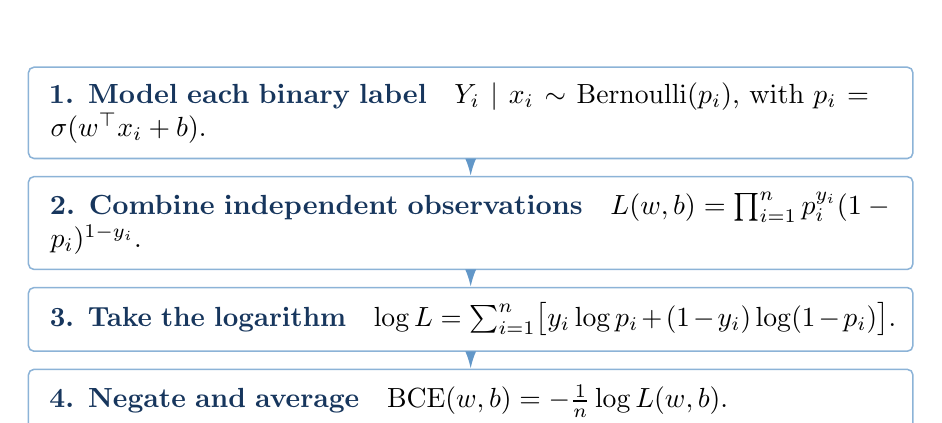
\begin{tikzpicture}[
  stage/.style={
    draw=blue!55,
    fill=white,
    rounded corners=2pt,
    line width=0.55pt,
    text width=0.88\linewidth,
    align=left,
    inner xsep=8pt,
    inner ysep=5.5pt
  },
  connector/.style={
    -{Latex[length=2.2mm,width=1.4mm]},
    draw=blue!75,
    line width=0.65pt
  }
]
\node[stage] (model) {%
  \textbf{\color{navy}1. Model each binary label}\quad
  $Y_i\mid x_i\sim\operatorname{Bernoulli}(p_i)$, with
  $p_i=\sigmoid(w^\top x_i+b)$.};
\node[stage, below=6pt of model] (likelihood) {%
  \textbf{\color{navy}2. Combine independent observations}\quad
  $L(w,b)=\prod_{i=1}^{n}p_i^{y_i}(1-p_i)^{1-y_i}$.};
\node[stage, below=6pt of likelihood] (loglikelihood) {%
  \textbf{\color{navy}3. Take the logarithm}\quad
  $\log L=\sum_{i=1}^{n}\bigl[y_i\log p_i+(1-y_i)\log(1-p_i)\bigr]$.};
\node[stage, below=6pt of loglikelihood] (loss) {%
  \textbf{\color{navy}4. Negate and average}\quad
  $\BCE(w,b)=-\frac{1}{n}\log L(w,b)$.};

\draw[connector] (model) -- (likelihood);
\draw[connector] (likelihood) -- (loglikelihood);
\draw[connector] (loglikelihood) -- (loss);
\end{tikzpicture}

\par\vspace{5pt}
\raggedright
\textbf{In words:} Bernoulli specifies each probability; independence creates the product; the logarithm converts that product to a sum; negation and averaging turn it into the loss minimized during training.
\end{keyidea}

\section{The shape of binary cross-entropy}

For a positive label $y=1$,
\[
\ell(1,p)=-\ln p.
\]
For a negative label $y=0$,
\[
\ell(0,p)=-\ln(1-p).
\]

\begin{figure}[htbp]
\centering
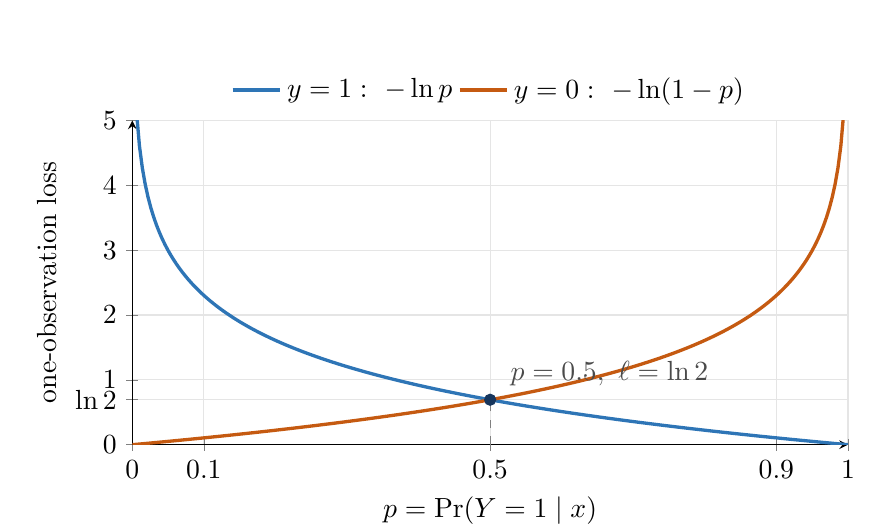
\begin{tikzpicture}
\begin{axis}[
  width=0.88\textwidth,
  height=0.47\textwidth,
  xmin=0,xmax=1,
  ymin=0,ymax=5,
  xlabel={$p=\Pr(Y=1\mid x)$},
  ylabel={one-observation loss},
  xtick={0,0.1,0.5,0.9,1},
  ytick={0,0.693,1,2,3,4,5},
  yticklabels={$0$,$\ln 2$,$1$,$2$,$3$,$4$,$5$},
  grid=major,
  grid style={draw=gray!20},
  axis lines=left,
  legend style={draw=none,fill=white,at={(0.5,1.02)},anchor=south,legend columns=2},
  clip=true
]
\addplot[blue,very thick,domain=0.006:1,samples=250] {-ln(x)};
\addlegendentry{$y=1:\ -\ln p$}
\addplot[orange,very thick,domain=0:0.994,samples=250] {-ln(1-x)};
\addlegendentry{$y=0:\ -\ln(1-p)$}
\addplot[only marks,mark=*,mark size=2pt,navy] coordinates {(0.5,0.693147)};
\draw[dashed,gray] (axis cs:0.5,0) -- (axis cs:0.5,0.693147);
\node[anchor=south west,text=graytext] at (axis cs:0.515,0.75) {$p=0.5,\ \ell=\ln 2$};
\end{axis}
\end{tikzpicture}
\caption{Binary cross-entropy as a function of the predicted class-1 probability. The two curves meet at $p=0.5$, but this is not a minimum. Each curve reaches loss 0 only when all probability is placed on its observed class.}
\label{fig:bce-curves}
\end{figure}

Important features of \cref{fig:bce-curves} are:
\begin{itemize}
  \item If $y=1$, the loss decreases toward 0 as $p\to1$ and diverges as $p\to0$.
  \item If $y=0$, the loss decreases toward 0 as $p\to0$ and diverges as $p\to1$.
  \item At $p=0.5$, both losses equal $-\ln(0.5)=\ln 2\approx0.693$. This is the crossing point and the point of maximum binary uncertainty, not the minimum of either curve.
  \item The theoretical range is $[0,\infty]$, with infinite loss when the model assigns probability zero to the outcome that occurs.
\end{itemize}

The divergence at a confidently wrong prediction is deliberate. A probabilistic model is making a much stronger and more falsifiable claim when it assigns probability $10^{-9}$ than when it assigns probability $0.4$ to an event that then occurs.

\section{A complete numerical example}

Suppose three independent observations have labels and predictions as follows:

\begin{center}
\begin{tabular}{ccccc}
\toprule
$i$ & $y_i$ & $p_i=\Pr(Y_i=1\mid x_i)$ & Probability of observed label $r_i$ & $-\ln r_i$ \\
\midrule
1 & 1 & 0.8 & 0.8 & 0.2231 \\
\rowrule
2 & 0 & 0.3 & $1-0.3=0.7$ & 0.3567 \\
\rowrule
3 & 1 & 0.6 & 0.6 & 0.5108 \\
\bottomrule
\end{tabular}
\end{center}

The joint likelihood is
\[
L=0.8\times0.7\times0.6=0.336.
\]
The negative log-likelihood is
\[
-\ln L=-\ln(0.336)=1.0906.
\]
The individual log losses add to the same value:
\[
0.2231+0.3567+0.5108=1.0906.
\]
The mean BCE is
\[
\frac{1.0906}{3}=0.3635.
\]
This example displays the entire product-to-sum relationship numerically.

\section{From probability loss to logit loss}

Substitute $p=\sigmoid(z)$ into the one-observation loss:
\begin{align}
\ell(z,y)
&=-y\log\sigmoid(z)-(1-y)\log(1-\sigmoid(z))\notag\\
&=\log(1+e^z)-yz\notag\\
&=\softplus(z)-yz.
\label{eq:softplus-loss}
\end{align}
Here $\softplus(z)=\log(1+e^z)$. This form reveals several useful mathematical properties.

\subsection{The gradient simplifies to \texorpdfstring{$p-y$}{p-y}}

Because
\[
\frac{d}{dz}\log(1+e^z)=\frac{e^z}{1+e^z}=\sigmoid(z)=p,
\]
we obtain
\begin{equation}
\boxed{\frac{\partial\ell}{\partial z}=p-y.}
\label{eq:gradient-logit}
\end{equation}
Using $z=w^\top x+b$ and the chain rule,
\begin{equation}
\nabla_w\ell=(p-y)x,
\qquad
\frac{\partial\ell}{\partial b}=p-y.
\label{eq:gradient-parameters}
\end{equation}

For example, if $y=1$ and $p=0.7$, then $p-y=-0.3$. Gradient descent subtracts a negative quantity, increasing $z$ and therefore increasing $p$. If $y=0$ and $p=0.7$, then $p-y=0.7$; gradient descent decreases $z$ and therefore decreases $p$.

\subsection{Convexity}

The second derivative with respect to the logit is
\begin{equation}
\frac{\partial^2\ell}{\partial z^2}=p(1-p)\ge0.
\label{eq:second-derivative}
\end{equation}
For a dataset, the Hessian with respect to $w$ has the form
\[
\nabla_w^2\operatorname{NLL}=X^\top W X,
\]
where $W$ is diagonal with entries $p_i(1-p_i)\ge0$. Hence the unregularized logistic-regression NLL is convex in its parameters. It may fail to be \emph{strictly} convex if the design matrix lacks rank or if other degeneracies are present.

Convexity means there are no inferior local minima in ordinary logistic regression. This favorable property belongs to the combination of a linear logit, sigmoid link, and Bernoulli negative log-likelihood.

\section[Cross-entropy, entropy, and KL divergence (optional)]{Cross-entropy, entropy, and KL divergence}
\label{sec:information-theory}

\begin{tcolorbox}[
  colback=lightgray,
  colframe=blue!55,
  boxrule=0.45pt,
  arc=1.5pt,
  left=6pt,right=6pt,top=4pt,bottom=4pt
]
\small
\textbf{\color{navy}Optional enrichment: information theory.}
This section gives the information-theoretic interpretation of binary cross-entropy. The later sections do not depend on it.
\end{tcolorbox}

The one-observation loss is a realized score. Cross-entropy in its population form averages that score over outcomes generated by a true distribution.

Let the true conditional probability of class 1 be $\pi$, while the model reports $p$. Then
\[
Q=(1-\pi,\pi),
\qquad
P=(1-p,p).
\]
The binary cross-entropy is
\begin{equation}
H(Q,P)
=\E_{Y\sim Q}[-\log P(Y)]
=-\pi\log p-(1-\pi)\log(1-p).
\label{eq:population-ce}
\end{equation}
This is the model's \emph{expected} surprisal when reality follows $Q$ but probabilities are quoted according to $P$.

The entropy of the true distribution is
\begin{equation}
H(Q)=-\pi\log\pi-(1-\pi)\log(1-\pi),
\label{eq:entropy}
\end{equation}
and the Kullback--Leibler divergence from $Q$ to $P$ is
\begin{equation}
\KL(Q\|P)
=\pi\log\frac{\pi}{p}
+(1-\pi)\log\frac{1-\pi}{1-p}.
\label{eq:kl}
\end{equation}
These quantities satisfy
\begin{equation}
\boxed{H(Q,P)=H(Q)+\KL(Q\|P).}
\label{eq:ce-decomposition}
\end{equation}
The entropy $H(Q)$ is the irreducible uncertainty inherent in the true outcome distribution. The nonnegative KL term is the extra expected log loss caused by using the wrong predictive distribution. Therefore, expected cross-entropy is minimized when $P=Q$, or $p=\pi$.

\subsection{Why log loss rewards honest probabilities}

For fixed true probability $\pi$, differentiate the expected loss in \cref{eq:population-ce} with respect to the reported probability $p$:
\[
\frac{\partial H(Q,P)}{\partial p}
=-\frac{\pi}{p}+\frac{1-\pi}{1-p}
=\frac{p-\pi}{p(1-p)}.
\]
The derivative is zero precisely at $p=\pi$, and this point is the unique minimum for $0<\pi<1$. The logarithmic score is therefore a \emph{strictly proper scoring rule}: in expectation, a forecaster does best by reporting its true probability rather than exaggerating or concealing uncertainty.

\begin{examplebox}[Single observation versus population]
If one observed label is $y=1$, the empirical point-mass distribution is $Q_y=(0,1)$, whose entropy is zero. Its cross-entropy with $P=(1-p,p)$ is simply $-\log p$. If repeated outcomes at the same $x$ truly have probability $\pi=0.7$, the population cross-entropy averages both possible labels and equals $-0.7\log p-0.3\log(1-p)$.
\end{examplebox}

In supervised learning, the sample mean in \cref{eq:bce-dataset} is an empirical estimate of expected cross-entropy under the data-generating distribution. This is why the same expression appears as both an average training loss and an information-theoretic quantity.

\section{Numerical stability}

The mathematical loss is intentionally unbounded, but a naive computer implementation can create avoidable infinities or undefined values.

\subsection{What goes wrong}

A naive implementation performs the following steps:
\[
z\longrightarrow p=\sigmoid(z)
\longrightarrow -y\log p-(1-y)\log(1-p).
\]
For a very negative $z$, finite-precision arithmetic may round $p$ to exactly 0. If $y=1$, the program evaluates $-\log 0=+\infty$. For a very positive $z$, $p$ may round to exactly 1, making $\log(1-p)$ problematic when $y=0$. In some implementations, the algebraic-looking inactive term $0\log0$ can also produce a `NaN' even though its mathematical limiting contribution should be zero.

\subsection{Stable BCE from logits}

The preferred approach is to combine the sigmoid and BCE algebraically and compute directly from $z$:
\begin{equation}
\boxed{
\ell(z,y)=\max(z,0)-zy+\log\left(1+e^{-|z|}\right).}
\label{eq:stable-bce}
\end{equation}
This expression is mathematically equivalent to \cref{eq:softplus-loss}, but it avoids exponentiating a large positive number and avoids forming probabilities that round to exactly 0 or 1. Major machine-learning libraries therefore provide operations commonly described as \emph{binary cross-entropy with logits} or \emph{sigmoid cross-entropy with logits}.

Clipping probabilities to $[\varepsilon,1-\varepsilon]$ is a simple fallback, but it changes the objective near the boundaries and can distort gradients. If logits are available, a stable fused logit formulation is preferable.

\begin{warningbox}[Two different numerical issues]
Taking the log of a full dataset likelihood prevents a product of many ordinary probabilities from underflowing. Computing BCE directly from logits prevents $\sigmoid(z)$ from rounding to 0 or 1 before a logarithm is taken. These are related but distinct uses of numerical stability.
\end{warningbox}

\section{Why not ordinary squared error?}

Squared error is not nonsensical for probability forecasts. The Brier score $(p-y)^2$ is also a strictly proper scoring rule. Nevertheless, BCE is the canonical loss for Bernoulli logistic regression because it is exactly the model's negative log-likelihood and has especially convenient optimization geometry.

\begin{center}
\begin{tabularx}{0.96\textwidth}{>{\raggedright\arraybackslash}p{0.22\textwidth}XX}
\toprule
& \textbf{Binary cross-entropy} & \textbf{Squared probability error} \\
\midrule
One-observation loss & $-y\log p-(1-y)\log(1-p)$ & $(p-y)^2$ \\
\rowrule
Statistical role & Bernoulli negative log-likelihood & Brier score; a different proper scoring rule \\
\rowrule
Gradient with respect to $z$ & $p-y$ & $2(p-y)p(1-p)$ \\
\rowrule
Confident wrong prediction & Unbounded penalty & Penalty bounded by 1 \\
\rowrule
Convex in linear-logit parameters & Yes & Not generally \\
\rowrule
Behavior at saturated sigmoid & Retains a large logit gradient when confidently wrong & Extra factor $p(1-p)$ can make the gradient very small \\
\bottomrule
\end{tabularx}
\end{center}

Thus BCE is not the only conceivable probability loss. Its special status comes from the conjunction of Bernoulli likelihood, logarithmic information, additive independent evidence, proper probabilistic scoring, and clean optimization.

\section{Assumptions, limitations, and extensions}

\subsection{Conditional independence does not mean independent features}

The likelihood product in \cref{eq:dataset-likelihood} assumes that the labels are independent \emph{conditional on} the observed predictors and model parameters. It does not require the components of $x$ to be independent. Repeated measurements, clustered observations, time series, and network data may violate the conditional-independence assumption and require a different likelihood or dependence model.

\subsection{Maximum likelihood depends on the model}

Maximum likelihood finds the best parameter inside the assumed model family. It does not guarantee that the family is correct, that omitted variables are harmless, or that predictions generalize. Model diagnostics, validation data, and domain knowledge remain necessary.

\subsection{Complete separation}

If a linear boundary perfectly separates the two classes, unregularized logistic regression may have no finite MLE: increasing the magnitude of $w$ can push every training probability closer to its observed label and drive the BCE toward zero without attaining a finite optimum. Regularization, such as an $L_2$ penalty, produces a finite solution and controls model complexity. A penalized objective is no longer pure maximum likelihood; with an appropriate prior interpretation, it can be viewed as maximum a posteriori estimation.

\subsection{Class weighting}

Weighted BCE is often used for unequal error costs or sampling designs:
\[
\ell_{\mathrm{weighted}}(y,p)
=-\left[\alpha y\log p+\beta(1-y)\log(1-p)\right].
\]
Weights change the target criterion and can change probability calibration. They should be chosen to match the inferential or decision objective, not merely because the classes have different frequencies.

\subsection{Multiclass extension}

For $K$ mutually exclusive classes, logistic regression generalizes to softmax regression. If $q_k$ is the true one-hot label distribution and $p_k$ is the model probability for class $k$, categorical cross-entropy is
\[
H(Q,P)=-\sum_{k=1}^{K}q_k\log p_k.
\]
Because $Q$ is one-hot, this again reduces to the negative log probability assigned to the observed class.

\section{Common misconceptions}

\begin{enumerate}[label=\textbf{\arabic*.}]
  \item \textbf{``BCE takes the logarithm of the prediction error.''}\\
  No. It takes the negative logarithm of the probability assigned to the observed outcome.

  \item \textbf{``The logarithm comes from the Bernoulli distribution.''}\\
  Not directly. Bernoulli supplies $p^y(1-p)^{1-y}$. The log is applied when forming an additive log-likelihood or logarithmic score.

  \item \textbf{``The minimum loss is at $p=0.5$.''}\\
  No. At $p=0.5$, the loss is $\ln2\approx0.693$ for either label. The minimum is 0 at $p=1$ when $y=1$ and at $p=0$ when $y=0$.

  \item \textbf{``The log is used only to avoid tiny likelihood products.''}\\
  Numerical stability matters, but the deeper reason is additivity: independent probabilities multiply while independent information should add.

  \item \textbf{``Natural logarithm is the only acceptable base.''}\\
  No. Any logarithm gives the same optimizer up to positive scaling. Base 2 yields bits; base $e$ yields nats and simpler calculus.

  \item \textbf{``Cross-entropy is classification accuracy.''}\\
  No. Accuracy sees only which side of a decision threshold wins. Cross-entropy evaluates the full reported probability and strongly distinguishes cautious from confident errors.

  \item \textbf{``Likelihood is the probability that the parameter is true.''}\\
  No. It is the probability of the observed data considered as a function of the parameter. A probability distribution over parameters belongs to Bayesian inference.

  \item \textbf{``The loss becoming infinite means the theory is broken.''}\\
  No. Infinite loss is the coherent logarithmic penalty for assigning probability zero to an event that occurs. Stable implementations keep finite logits computable without pretending the theoretical boundary is harmless.
\end{enumerate}

\section{Terminology reference}

\begin{description}[style=nextline,font=\normalfont\bfseries]
  \item[Bernoulli distribution] A probability model for one binary outcome, parameterized by $p=\Pr(Y=1)$.
  \item[Binary cross-entropy (BCE)] The average or expected negative logarithmic score for binary outcomes.
  \item[Calibration] Agreement between predicted probabilities and long-run event frequencies; among cases predicted near 0.7, roughly 70\% should be positive in a well-calibrated model.
  \item[Conditional independence] Independence after conditioning on specified variables and parameters; the standard assumption that permits the logistic-regression likelihood to factor over observations.
  \item[Entropy] Expected self-information under the same distribution that generates and scores outcomes: $H(Q)=\E_Q[-\log Q(Y)]$.
  \item[Cross-entropy] Expected self-information when outcomes come from $Q$ but are scored using probabilities from $P$: $H(Q,P)=\E_Q[-\log P(Y)]$.
  \item[KL divergence] The nonnegative excess cross-entropy due to using $P$ instead of $Q$: $\KL(Q\|P)=H(Q,P)-H(Q)$.
  \item[Likelihood] The probability of the observed data, regarded as a function of unknown model parameters.
  \item[Logit] The log-odds $\log[p/(1-p)]$; in logistic regression it equals $w^\top x+b$.
  \item[Log-likelihood] The logarithm of the likelihood; it converts products across observations into sums.
  \item[Maximum likelihood estimate (MLE)] The parameter value maximizing the likelihood, equivalently the log-likelihood.
  \item[Negative log-likelihood (NLL)] The negative log-likelihood, written as a minimization objective. For Bernoulli observations it is summed BCE.
  \item[Proper scoring rule] A probability scoring rule whose expected value is optimized by reporting the true probability; log loss and the Brier score are examples.
  \item[Sigmoid] The inverse-logit mapping $\sigmoid(z)=1/(1+e^{-z})$, which maps any real score to $(0,1)$.
  \item[Surprisal / self-information] The realized information $-\log p$ associated with observing an event assigned probability $p$.
\end{description}

\section{Summary}

The core ideas can be compressed into six statements:
\begin{enumerate}
  \item Logistic regression models $Y\mid x$ as Bernoulli with probability $p=\sigmoid(w^\top x+b)$.
  \item The Bernoulli formula gives the observed label probability $p^y(1-p)^{1-y}$.
  \item Conditional independence makes dataset likelihood contributions multiply.
  \item Requiring independent information to add leads essentially uniquely to $-\log p$; the logarithm also turns the likelihood product into a sum without changing its maximizer.
  \item The resulting Bernoulli negative log-likelihood is binary cross-entropy, and its logit derivative is the simple residual $p-y$.
  \item Stable software computes the loss directly from logits, not by separately forming a possibly rounded probability and then taking its logarithm.
\end{enumerate}

The deepest conceptual point is therefore not that a logarithm was arbitrarily attached to an error. The model assigns probabilities through a conditional Bernoulli distribution; maximum likelihood asks those probabilities to support the observed data; and logarithmic information is the additive language in which independent probabilistic evidence is naturally measured.

\clearpage
\appendix

\section{Manifestations of BCE Across Machine-Learning Algorithms}
\label{app:bce-manifestations}

Binary cross-entropy is not tied to one algorithm. It is tied to a \emph{probability model}: somewhere in the learning problem, an outcome is represented as a Bernoulli event and the model produces a probability for that event. Logistic regression is the simplest example, but the logit can be produced by a neural network, an additive ensemble of trees, a matrix-factorization model, or another function approximator.

\begin{keyidea}[Terminology: BCE and BCE loss]
\emph{Binary cross-entropy} and \emph{binary cross-entropy loss} normally refer to the same objective. The common forms are \textbf{BCE} and \textbf{BCE loss}; the latter is linguistically redundant but conventional in software documentation.
\end{keyidea}

\subsection{One mathematical template}

Suppose a learning problem contains binary targets indexed by pairs $(i,j)$, where $i$ identifies an observation and $j$ might identify a label, pixel, item, time interval, or detection candidate. A model produces logits
\[
z_{ij}=f_\theta(x_i)_j,
\qquad
p_{ij}=\sigmoid(z_{ij}),
\]
and applies the elementwise Bernoulli loss
\begin{equation}
\ell_{ij}
=-y_{ij}\log p_{ij}-(1-y_{ij})\log(1-p_{ij}).
\label{eq:appendix-general-bce}
\end{equation}
Training aggregates the applicable terms:
\begin{equation}
\mathcal L(\theta)
=\frac{1}{|\mathcal I|}
\sum_{(i,j)\in\mathcal I}\ell_{ij},
\label{eq:appendix-bce-reduction}
\end{equation}
possibly with weights or masks. The same loss therefore takes on different practical meanings according to:
\begin{enumerate}
  \item what binary event $y_{ij}$ represents;
  \item how the algorithm constructs the logit $z_{ij}$; and
  \item whether BCE is the direct training objective, a local split criterion, or only an evaluation metric.
\end{enumerate}

Using a sum of elementwise BCE terms amounts to a factorized Bernoulli likelihood for those targets, at least as a working objective. That factorization may be an exact scientific assumption, a useful conditional approximation, or simply a surrogate training criterion. These interpretations should not be silently conflated.

\clearpage
\thispagestyle{fancy}
\subsection{Direct uses of BCE}

\small
\begin{longtable}{>{\raggedright\arraybackslash}p{0.19\textwidth}>{\raggedright\arraybackslash}p{0.21\textwidth}>{\raggedright\arraybackslash}p{0.48\textwidth}}
\caption{Common direct uses of binary cross-entropy.}\label{tab:bce-direct-uses}\\
\toprule
\textbf{Setting} & \textbf{Binary event} & \textbf{How BCE manifests} \\
\midrule
\endfirsthead
\multicolumn{3}{l}{\small\itshape Table \thetable\ continued from the previous page.}\\
\toprule
\textbf{Setting} & \textbf{Binary event} & \textbf{How BCE manifests} \\
\midrule
\endhead
\midrule
\multicolumn{3}{r}{\small\itshape Continued on the next page.}\\
\endfoot
\bottomrule
\endlastfoot

Classical logistic regression
& Entire observation is class 1 or 0
& The logit is linear, $z=w^\top x+b$. BCE is exactly the conditional Bernoulli NLL. \\
\rowrule

Binary neural-network classifier
& Entire observation is positive or negative
& A nonlinear network produces features and a final scalar logit. The output layer is logistic regression on learned features. \\
\rowrule

Multi-label classification
& Attribute $j$ is present or absent
& The model produces one sigmoid per label and sums or averages BCE across labels. Labels need not be mutually exclusive, unlike softmax classes. \\
\rowrule

Binary semantic segmentation
& Pixel $j$ belongs or does not belong to a target region
& A convolutional or transformer model produces a logit for each pixel. Pixelwise BCE is often combined with Dice- or overlap-based losses. \\
\rowrule

Object detection
& An object is present at a candidate location, or an independent class is present
& BCE can score objectness and independent class outputs. Class imbalance often motivates weighting or focal loss. \\
\rowrule

Click-through and conversion prediction
& User clicks, purchases, or converts
& A linear model, neural model, or factorization model produces an interaction logit. BCE is the event NLL when the training sample reflects the intended population. \\
\rowrule

Implicit-feedback recommendation
& User interacts or does not interact with an item
& Positive interactions and sampled negatives are trained with logistic terms. Negative sampling changes the sampled class distribution, so raw scores need not be calibrated population probabilities. \\
\rowrule

Bernoulli decoder or autoencoder
& A reconstructed bit or binary feature equals 1 or 0
& Decoder outputs parameterize Bernoulli observations. This likelihood is natural for binary data, but it may be a poor observation model for genuinely continuous measurements. \\
\rowrule

Classic GAN discriminator
& Input is real or generated
& The discriminator is trained as a binary classifier with logarithmic loss. Common generator objectives use related log terms but have a different optimization role \cite{goodfellow2014}. \\
\rowrule

Discrete-time survival model
& An event occurs or does not occur during interval $j$, conditional on survival to that interval
& Interval-specific sigmoid outputs estimate hazards. The observed or censored survival likelihood decomposes into BCE-like event and non-event terms over the intervals at risk. \\
\rowrule

Negative-sampling objectives
& A data pair is observed or sampled from a noise distribution
& Logistic discrimination between positive and sampled negative pairs produces a sum of BCE-like log-sigmoid terms; word-embedding objectives provide a familiar example \cite{mikolov2013}. \\
\end{longtable}
\normalsize

The phrase ``BCE is used'' is strongest when \cref{eq:appendix-bce-reduction} is the explicit objective. It is weaker when an algorithm merely produces probabilities that are later evaluated by BCE.

\subsection{Ordinary decision trees: entropy as fitted leaf BCE}
\label{app:ordinary-trees}
\thispagestyle{fancy}

Consider a candidate tree node containing $n_1$ positive and $n_0$ negative observations, with $n=n_0+n_1$ and positive fraction
\[
q=\frac{n_1}{n}.
\]
If the node becomes a leaf and predicts one constant probability $p$ for all of its observations, its total BCE is
\begin{equation}
\mathcal L_{\mathrm{node}}(p)
=-n_1\log p-n_0\log(1-p).
\label{eq:node-bce}
\end{equation}
Differentiating shows that the best constant probability is the empirical class fraction:
\[
\frac{d\mathcal L_{\mathrm{node}}}{dp}
=-\frac{n_1}{p}+\frac{n_0}{1-p}=0
\quad\Longrightarrow\quad
\widehat p=q.
\]
At this fitted value, the average BCE in the node is
\begin{equation}
\frac{1}{n}\mathcal L_{\mathrm{node}}(\widehat p)
=-q\log q-(1-q)\log(1-q)
=H(q),
\label{eq:node-entropy-bce}
\end{equation}
which is exactly binary entropy.

For a proposed split into left and right children, entropy-based information gain is
\begin{equation}
\Delta H
=H(q_{\mathrm{parent}})
-\frac{n_L}{n}H(q_L)
-\frac{n_R}{n}H(q_R).
\label{eq:tree-information-gain}
\end{equation}
Consequently, maximizing information gain is equivalent to maximizing the reduction in training BCE obtained when the parent and candidate children each use their own fitted constant probability. This explains the precise link between the entropy split criterion and BCE in classification trees \cite{breiman1984}.

There are two important qualifications:
\begin{itemize}
  \item This is a \emph{local greedy split calculation}. An ordinary decision tree does not differentiate a smooth, global BCE objective through every possible tree topology.
  \item Many trees use Gini impurity, $1-q^2-(1-q)^2=2q(1-q)$, rather than entropy. Gini and entropy have similar qualitative shapes, but Gini is not BCE and contains no logarithm.
\end{itemize}

\subsection{Random forests and probability evaluation}

A random forest trains many trees on perturbed data and feature sets, then averages their class votes or leaf probabilities. Depending on the implementation, each tree may use entropy, Gini impurity, or another split rule. The forest therefore does not usually minimize one global BCE objective.

Nevertheless, BCE remains relevant in three ways:
\begin{enumerate}
  \item an entropy-trained constituent tree uses the local relationship in \cref{eq:node-entropy-bce};
  \item the forest's final probabilities can be selected or evaluated using held-out log loss; and
  \item calibration methods can be applied when averaged tree probabilities are systematically too sharp or too conservative.
\end{enumerate}

A raw leaf estimate $\widehat p=n_1/n$ can equal exactly 0 or 1. It gives zero training loss in a pure leaf but infinite test log loss if the opposite class later appears. The symmetric Beta smoothing rule $\widetilde p=(n_1+\alpha)/(n+2\alpha)$ keeps estimates away from the boundaries. Common choices include $\alpha=1$ for Laplace smoothing and $\alpha=1/2$ for Jeffreys smoothing. Cross-validation or a dedicated calibration set is preferable when enough data are available.

\subsection{Gradient-boosted trees: direct optimization of BCE}
\label{app:boosted-trees}

Binary gradient boosting constructs an additive \emph{logit} model
\begin{equation}
F_M(x)=F_0(x)+\sum_{m=1}^{M}\eta f_m(x),
\qquad
p(x)=\sigmoid(F_M(x)),
\label{eq:boosted-logit}
\end{equation}
where each $f_m$ is a regression tree and $\eta$ is a learning rate. The ensemble can directly minimize
\[
\sum_{i=1}^{n}\left[-y_i\log p_i-(1-y_i)\log(1-p_i)\right].
\]
For the current logit $F(x_i)$, the first and second derivatives are
\begin{equation}
g_i=p_i-y_i,
\qquad
h_i=p_i(1-p_i).
\label{eq:boosted-derivatives}
\end{equation}
First-order boosting fits a new tree to approximate the negative gradient $y_i-p_i$. Newton-style boosting uses both $g_i$ and $h_i$ to form split gains and leaf updates. This is a direct algorithmic manifestation of the same $p-y$ gradient derived for logistic regression. The difference is that the logit function is now built from trees rather than restricted to a linear form \cite{friedman2001,chen2016}.

\begin{center}
\begin{tabularx}{0.96\textwidth}{>{\raggedright\arraybackslash}p{0.23\textwidth}>{\raggedright\arraybackslash}p{0.25\textwidth}X}
\toprule
\textbf{Tree method} & \textbf{Relationship to BCE} & \textbf{Key distinction} \\
\midrule
Entropy classification tree & Local equivalence & Split gain equals reduction in fitted node BCE. \\
\rowrule
Gini classification tree & Indirect / none algebraically & Similar impurity goal, but no logarithmic loss. \\
\rowrule
Random forest & Usually evaluation-level & Trees are bagged; the ensemble generally has no single global BCE training objective. \\
\rowrule
Logistic gradient boosting & Direct global objective & Trees add corrections to logits using BCE gradients, and often Hessians. \\
\rowrule
AdaBoost & Different objective & Classical AdaBoost is associated with exponential loss, not BCE. \\
\bottomrule
\end{tabularx}
\end{center}

\subsection{Multi-label learning versus multiclass learning}

This distinction is a frequent source of implementation errors.

\paragraph{Multi-label problem.}
Several labels may simultaneously be true, such as an image containing both a dog and a car. The model uses independent sigmoid outputs and elementwise BCE:
\[
p_k=\sigmoid(z_k),
\qquad
\mathcal L=-\sum_{k=1}^{K}\left[y_k\log p_k+(1-y_k)\log(1-p_k)\right].
\]
The probabilities do not need to sum to 1.

\paragraph{Single-label multiclass problem.}
Exactly one of $K$ classes is true, such as a digit being exactly one of 0 through 9. The usual model uses a softmax distribution
\[
p_k=\frac{e^{z_k}}{\sum_{r=1}^{K}e^{z_r}},
\qquad
\sum_{k=1}^{K}p_k=1,
\]
and categorical cross-entropy. Applying independent BCE terms instead changes the probabilistic model. A one-vs-rest construction can sometimes be useful, but its outputs are not automatically a coherent mutually exclusive probability distribution.

\subsection{Weighted BCE, focal loss, masks, and soft targets}

Many practical objectives are modifications of BCE rather than the plain Bernoulli NLL.

\paragraph{Weighted BCE.}
Different costs or sampling weights can be represented as
\begin{equation}
\ell_{\mathrm{weighted}}
=-\alpha y\log p-\beta(1-y)\log(1-p).
\label{eq:appendix-weighted-bce}
\end{equation}
This can emphasize rare positives or asymmetric errors, but arbitrary weighting changes the population objective. If calibrated probabilities are required, class-prior changes and sampling weights must be handled deliberately.

\paragraph{Focal loss.}
Define the probability assigned to the observed class as
\[
p_t=yp+(1-y)(1-p).
\]
Binary focal loss is
\begin{equation}
\operatorname{FL}(p_t)
=-\alpha_t(1-p_t)^\gamma\log p_t.
\label{eq:focal-loss}
\end{equation}
The factor $(1-p_t)^\gamma$ downweights already-easy examples and concentrates learning on difficult ones. With $\gamma=0$, focal loss reduces to weighted BCE. It is widely associated with dense object detection \cite{lin2017}.

\paragraph{Masked BCE.}
If only some targets are observed or meaningful, a mask $m_{ij}\in\{0,1\}$ limits the reduction to valid elements:
\[
\mathcal L
=\frac{\sum_{i,j}m_{ij}\ell_{ij}}
{\sum_{i,j}m_{ij}}.
\]
This is common for padded sequences, partially annotated labels, and spatial regions that should be ignored.

\paragraph{Soft targets.}
The algebra permits $y\in[0,1]$ rather than only $\{0,1\}$. Such targets can encode label smoothing, uncertain annotations, distillation probabilities, or mixtures of examples. In that case the term is cross-entropy between two Bernoulli distributions rather than the NLL contribution of one hard observed label.

\clearpage
\thispagestyle{fancy}
\subsection{When BCE is not the appropriate likelihood}

BCE should be chosen because the output represents a Bernoulli event or because logarithmic binary scoring is deliberately desired, not merely because the word ``classification'' appears in the problem.

\begin{center}
\begin{tabularx}{0.96\textwidth}{>{\raggedright\arraybackslash}p{0.30\textwidth}>{\raggedright\arraybackslash}p{0.28\textwidth}X}
\toprule
\textbf{Outcome structure} & \textbf{Typical model or loss} & \textbf{Why plain BCE may be unsuitable} \\
\midrule
One of $K>2$ mutually exclusive classes & Softmax categorical cross-entropy & Independent Bernoulli outputs do not enforce probabilities summing to 1. \\
\rowrule
Count data & Poisson or negative-binomial NLL & Counts are not binary outcomes. \\
\rowrule
Continuous measurements & Gaussian NLL / squared error, or another continuous likelihood & A Bernoulli observation model has the wrong support. \\
\rowrule
Margin-based classification & Hinge loss & The goal is a separating margin rather than a calibrated Bernoulli likelihood. \\
\rowrule
Classical AdaBoost & Exponential loss & Its stagewise derivation uses a different surrogate objective. \\
\rowrule
Ranking & Pairwise or listwise ranking loss & The target concerns relative ordering rather than an isolated binary probability. \\
\rowrule
Dependent structured outputs & Structured likelihood or task-specific loss & Independent elementwise BCE may ignore essential dependence among outputs. \\
\bottomrule
\end{tabularx}
\end{center}

\subsection{Evaluation and interpretation across algorithms}

BCE can evaluate any model that outputs binary probabilities, even if BCE was not its training objective. This includes random forests, Bayesian models, nearest-neighbor probability estimates, and calibrated margin classifiers. However, several cautions apply:

\begin{itemize}
  \item \textbf{Accuracy and BCE answer different questions.} Accuracy evaluates thresholded decisions; BCE evaluates the entire probability assignment.
  \item \textbf{AUC and BCE answer different questions.} AUC primarily measures ranking; BCE is sensitive to probability calibration as well as discrimination.
  \item \textbf{The prevalence baseline matters.} A constant model predicting the positive fraction $q$ has average BCE $H(q)$. Loss values from datasets with different prevalences are therefore not automatically comparable.
  \item \textbf{Sampling can alter probability meaning.} Case-control sampling, negative sampling, or rebalancing can yield useful classifiers while shifting the relationship between raw scores and population probabilities.
  \item \textbf{Boundary probabilities are hazardous.} Predictions of exactly 0 or 1 receive infinite loss when contradicted. Stable logit computation addresses arithmetic failure; smoothing and calibration address overly extreme statistical estimates.
\end{itemize}

\begin{keyidea}[A useful classification of BCE manifestations]
Across machine learning, BCE plays four distinguishable roles:
\begin{enumerate}
  \item \textbf{Exact likelihood:} Bernoulli logistic regression, Bernoulli neural outputs, and discrete hazards.
  \item \textbf{Direct surrogate objective:} logistic gradient boosting, binary discrimination, and some negative-sampling objectives.
  \item \textbf{Local impurity measure:} entropy-based classification-tree splitting.
  \item \textbf{Evaluation score:} assessment of probabilistic predictions from almost any binary classifier.
\end{enumerate}
Recognizing the role prevents an important category error: the same numerical formula can be an assumed data likelihood in one algorithm, an optimization surrogate in another, and merely an external score in a third.
\end{keyidea}

\small
\begin{thebibliography}{99}

\bibitem{shannon1948}
C. E. Shannon,
``A Mathematical Theory of Communication,''
\emph{Bell System Technical Journal}, vol. 27, pp. 379--423 and 623--656, 1948.

\bibitem{bishop2006}
C. M. Bishop,
\emph{Pattern Recognition and Machine Learning}.
Springer, 2006.

\bibitem{hastie2009}
T. Hastie, R. Tibshirani, and J. Friedman,
\emph{The Elements of Statistical Learning}, 2nd ed.
Springer, 2009.

\bibitem{goodfellow2016}
I. Goodfellow, Y. Bengio, and A. Courville,
\emph{Deep Learning}.
MIT Press, 2016.

\bibitem{murphy2022}
K. P. Murphy,
\emph{Probabilistic Machine Learning: An Introduction}.
MIT Press, 2022.

\bibitem{breiman1984}
L. Breiman, J. H. Friedman, R. A. Olshen, and C. J. Stone,
\emph{Classification and Regression Trees}.
Wadsworth, 1984.

\bibitem{friedman2001}
J. H. Friedman,
``Greedy Function Approximation: A Gradient Boosting Machine,''
\emph{The Annals of Statistics}, vol. 29, no. 5, pp. 1189--1232, 2001.

\bibitem{chen2016}
T. Chen and C. Guestrin,
``XGBoost: A Scalable Tree Boosting System,''
in \emph{Proceedings of the 22nd ACM SIGKDD International Conference on Knowledge Discovery and Data Mining}, pp. 785--794, 2016.

\bibitem{goodfellow2014}
I. Goodfellow, J. Pouget-Abadie, M. Mirza, B. Xu, D. Warde-Farley,
S. Ozair, A. Courville, and Y. Bengio,
``Generative Adversarial Nets,''
in \emph{Advances in Neural Information Processing Systems 27}, 2014.

\bibitem{mikolov2013}
T. Mikolov, I. Sutskever, K. Chen, G. S. Corrado, and J. Dean,
``Distributed Representations of Words and Phrases and their Compositionality,''
in \emph{Advances in Neural Information Processing Systems 26}, 2013.

\bibitem{lin2017}
T.-Y. Lin, P. Goyal, R. Girshick, K. He, and P. Doll\'ar,
``Focal Loss for Dense Object Detection,''
in \emph{Proceedings of the IEEE International Conference on Computer Vision}, pp. 2980--2988, 2017.

\end{thebibliography}
\normalsize

\end{document}
